\subsubsection{2.1. Thu thập và xây dựng tập dữ liệu }

\textit{2.1.1. Nguồn dữ liệu và phạm vi nghiên cứu}\vspace{0.2cm}

\indent Để xây dựng một hệ thống phát hiện Sybil có khả năng tổng quát hóa cao, quy trình thu thập dữ liệu được thiết kế để khai thác triệt để các tương tác xã hội thực tế trên quy mô lớn. Phần này trình bày chi tiết về hạ tầng khai thác dữ liệu và các phạm vi thời gian thực nghiệm được lựa chọn.\vspace{0.3cm}

Đề tài thực hiện khai thác dữ liệu từ \textbf{Lens Protocol} — một mạng xã hội phi tập trung vận hành trên mạng lưới chuỗi khối Lens Chain. Toàn bộ dữ liệu thô được truy vấn trực tiếp từ kho lưu trữ dữ liệu công khai thông qua \textbf{Google BigQuery} với bộ dữ liệu \texttt{lens-protocol-mainnet}.\vspace{0.3cm}

Để đánh giá hiệu quả của đề tài trên các mật độ dữ liệu khác nhau, đề tài thiết lập 03 phạm vi thời gian thu thập dữ liệu độc lập. Chi tiết các mốc thời gian được trình bày tại \textbf{Bảng \ref{tab:TimeScopes}} dưới đây.

\begin{table}[H]
    \centering
    \caption{Các phạm vi thời gian thu thập dữ liệu thực nghiệm}
    \label{tab:TimeScopes}
    \setlength{\tabcolsep}{10pt}
    \renewcommand{\arraystretch}{1.3}
    \begin{tabular}{|l|c|l|}
        \hline
        \textbf{Phạm vi} & \textbf{Khoảng thời gian} & \textbf{Ý nghĩa thực nghiệm} \\ \hline
        Theo Tuần & 01/12/2025 -- 07/12/2025 & Nhận diện các đợt tấn công chớp nhoáng. \\ \hline
        Theo Tháng & 01/12/2025 -- 31/12/2025 & Theo dõi tính duy trì hành vi xã hội. \\ \hline
        Theo Quý & 01/10/2025 -- 31/12/2025 & Quan sát cấu trúc đồ thị ổn định dài hạn. \\ \hline
    \end{tabular}
\end{table}

Quy trình trích xuất dữ liệu với \textbf{Google BigQuery} được thực hiện chặt chẽ dựa trên các đặc tả kỹ thuật của Lens Protocol. Toàn bộ các câu lệnh SQL đều áp dụng ràng buộc thời gian nghiêm ngặt dựa trên trường \texttt{created\_on} để giới hạn chính xác phạm vi nghiên cứu trong các phạm vi thời gian đã định. Đồng thời, nhằm tối ưu hóa cấu trúc đồ thị đa tầng và nâng cao chất lượng học biểu diễn, hệ thống thực hiện lọc bỏ các nút cô lập — những tài khoản không phát sinh bất kỳ liên kết nào với các tài khoản còn lại trong khung thời gian khảo sát. Thao tác này không chỉ là một thủ tục kỹ thuật nhằm tối ưu hóa tài nguyên tính toán, mà còn dựa trên nền tảng triết lý về tính chuẩn hóa trong thực nghiệm GNN của Shchur và cộng sự \cite{shchur2018pitfalls}. Theo quan điểm của nghiên cứu này, việc giữ lại các nút cô lập trong tập dữ liệu thực nghiệm có thể dẫn đến "pha loãng" kết quả đánh giá, làm lu mờ sức mạnh thực sự của các hàm tổng hợp láng giềng — vốn là giá trị cốt lõi của cơ chế truyền tin. Đối với hệ thống \textbf{SybilSignal}, bước chuẩn hóa này đóng vai trò giúp các mô hình có thể đưa ra các dự đoán dựa trên tri thức cấu trúc mạng lưới thay vì chỉ phụ thuộc vào các thuộc tính định danh đơn thuần.\vspace{0.3cm}

Kết quả định lượng của quá trình tinh lọc này trên ba phạm vi thời gian nghiên cứu được minh họa chi tiết tại \textbf{Hình \ref{fig:NodeFilteringStats}}. Qua đó, có thể thấy số lượng tài khoản có phát sinh hành vi xã hội chiếm tỷ lệ đáng kể, tạo nên một mạng lưới liên kết đủ dày đặc để thực hiện các phân tích đồ thị chuyên sâu.\vspace{0.3cm}

\begin{figure}[H]
    \centering
    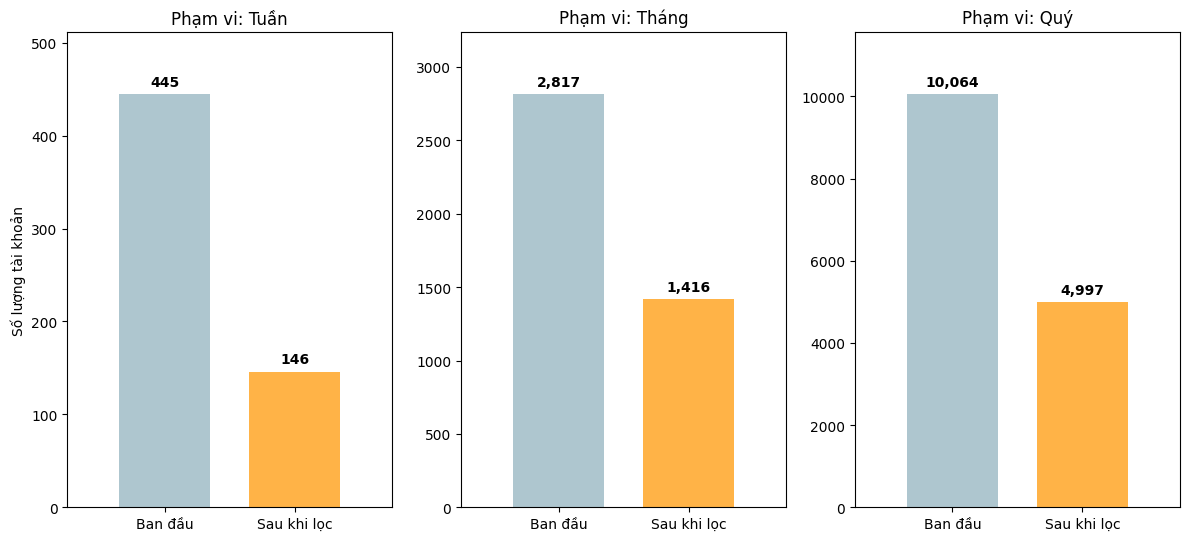
\includegraphics[width=\linewidth]{images/part-02/chap-02/sec-02/NodeFilteringStats.png}
    \caption{Thống kê số lượng Profile ban đầu và sau khi lọc nút cô lập}
    \label{fig:NodeFilteringStats}
\end{figure}

% =========================================================================================

\textit{2.1.2. Thống kê và đặc tả cấu trúc dữ liệu đồ thị đa tầng}\vspace{0.2cm}

Sau bước tiền lọc các nút cô lập, tập dữ liệu thu được mang những đặc tính đa tầng, phản ánh các khía cạnh hành vi khác nhau trong không gian mạng xã hội phi tập trung. Phần này thực hiện phân tích về quy mô quan hệ và chất lượng thuộc tính nút nhằm thiết lập nền tảng cho việc xây dựng các đặc trưng huấn luyện mô hình.\vspace{0.3cm}

\textbf{a. Quy mô quan hệ đa tầng}\vspace{0.2cm}

Mạng lưới hành vi trong hệ thống \textbf{SybilSignal} được đặc tả qua bốn tầng quan hệ chính: Theo dõi, Tương tác, Tương đồng và Đồng sở hữu. Kết quả thống kê số lượng cạnh sau khi đã thực hiện tạo cạnh đối xứng cho các quan hệ có hướng được trình bày tại \textbf{Hình \ref{fig:MultiLayerEdges}}.

\begin{figure}[H]
    \centering
    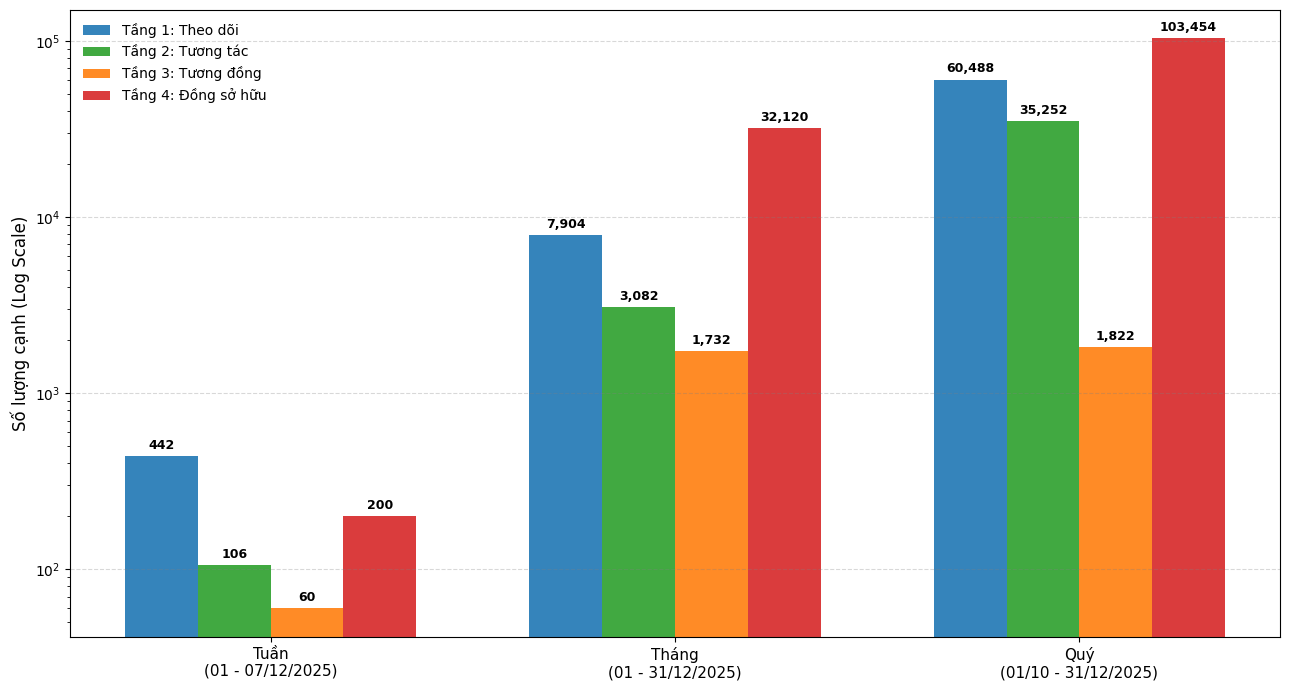
\includegraphics[width=\linewidth]{images/part-02/chap-02/sec-02/MultiLayerEdgesDistribution.png}
    \caption{Phân bổ số lượng cạnh trên bốn tầng đồ thị qua các phạm vi thời gian}
    \label{fig:MultiLayerEdges}
\end{figure}

Dữ liệu cho thấy sự tăng trưởng quy mô cạnh theo cấp số nhân khi mở rộng phạm vi nghiên cứu. Đặc biệt, tầng \textit{Đồng sở hữu} thể hiện sự bùng nổ về số lượng cạnh tại phạm vi Quý với $103,454$ liên kết, cao gấp hơn 500 lần so với phạm vi Tuần ($200$ cạnh). Điều này minh chứng cho sự tồn tại của các cụm Sybil có mối liên kết chặt chẽ về tính sở hữu, vốn là một trong những tín hiệu quan trọng nhất để nhận diện mạng lưới Sybil chuyên nghiệp hoạt động dài hạn.\vspace{0.3cm}

\textbf{b. Chất lượng và đặc trưng thuộc tính văn bản}\vspace{0.2cm}

Chất lượng dữ liệu định danh đóng vai trò quyết định đến hiệu quả của quá trình nhúng ngữ nghĩa (\textit{Node Embedding}). Đề tài thực hiện đánh giá hai chỉ số then chốt: Tỷ lệ lấp đầy và Độ dài văn bản trung bình trên ba trường dữ liệu: \texttt{handle}, \texttt{display\_name} và \texttt{bio}.

\begin{figure}[H]
    \centering
    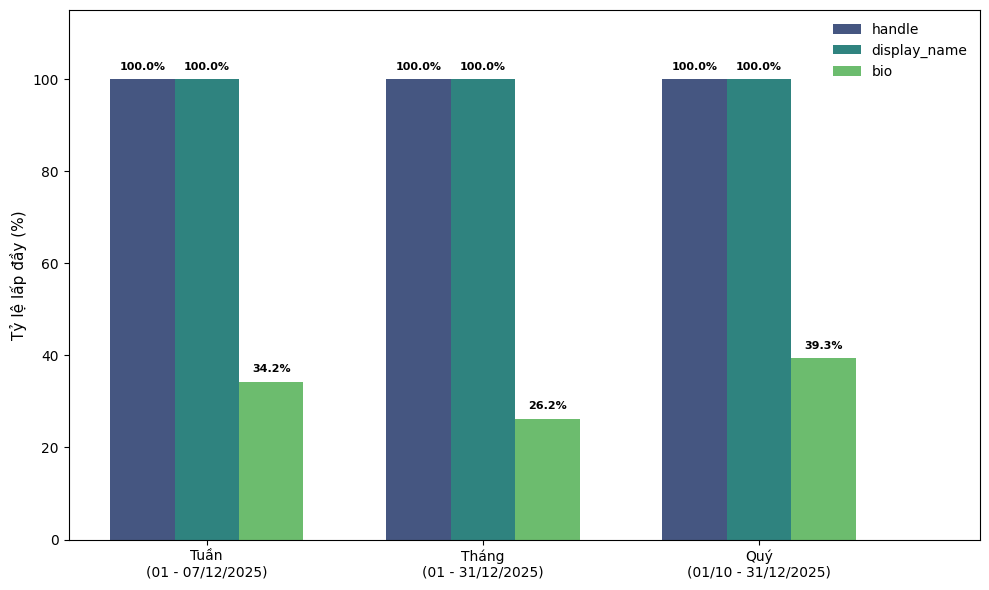
\includegraphics[width=\linewidth]{images/part-02/chap-02/sec-02/NodeAttributeFillRate.png}
    \caption{Thống kê tỷ lệ lấp đầy dữ liệu của các trường thuộc tính nút}
    \label{fig:NodeFillRate}
\end{figure}

Kết quả tại \textbf{Hình \ref{fig:NodeFillRate}} cho thấy trong khi \texttt{handle} và \texttt{display\_name} có tỷ lệ lấp đầy tuyệt đối, trường \texttt{bio} lại có độ thưa thớt cao (dao động từ 26.2\% đến 39.3\%). Trong nghiên cứu này, quá trình xây dựng đặc trưng thực hiện ghép nối các trường dữ liệu bao gồm \texttt{handle}, \texttt{display\_name} và \texttt{bio} thành một chuỗi văn bản tổng hợp duy nhất phục vụ cho mô hình nhúng. Mật độ thông tin sau khi ghép nối này được minh họa rõ nét tại \textbf{Hình \ref{fig:FeatureStringLengthStacked}} thông qua độ dài trung bình.

\begin{figure}[H]
    \centering
    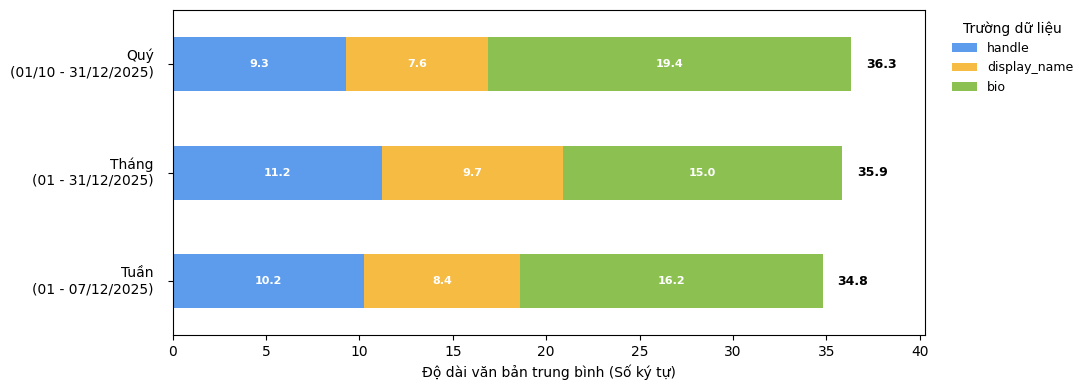
\includegraphics[width=\linewidth]{images/part-02/chap-02/sec-02/FeatureStringLengthStacked.png}
    \caption{Phân bổ độ dài văn bản trung bình trong chuỗi đặc trưng tổng hợp}
    \label{fig:FeatureStringLengthStacked}
\end{figure}

Bằng cách kết hợp các trường dữ liệu, độ dài chuỗi đầu vào cho mô hình nhúng ngữ nghĩa được duy trì ổn định ở mức xấp xỉ 35 ký tự (Ví dụ phạm vi Quý đạt 36.3 ký tự, trong đó đóng góp từ \texttt{bio} là 19.4). Việc duy trì một "vân tay văn bản" đủ dày giúp mô hình \textbf{all-MiniLM-L6-v2} có thể trích xuất các vector đặc trưng có độ phân tách cao, ngay cả đối với các nút có thuộc tính mô tả bị khuyết thiếu.\vspace{0.3cm}

Tổng kết lại, các con số thống kê thô cho thấy tập dữ liệu đã hội đủ các điều kiện cần thiết về quy mô liên kết và độ phong phú đặc trưng trên cả 3 phạm vi dữ liệu để tiến hành các bước tiền xử lý tiếp theo.